\subsection{Desenvolver Suíte de Testes Automatizados}

A suíte de testes automatizados possui a responsabilidade de garantir o correto funcionamento da integração entre os sistemas envolvidos, ou seja prover um meio onde possa ser testado tanto o Webservice do GSAN quanto a \textit{interface} Agi implementada para o Asterisk, para essa situação foram utilizados recursos do JUnit para criação dos cenários de teste, execução dos testes e identificação de falhas, quanto recursos do \textit{framework} Asterisk-Java para simular e controlar chamadas telefônicas com parametrização dinâmica.   

Os testes criados utilizando o \textit{framework} JUnit, podem ser executados a qualquer momento, seja manualmente pela própria IDE de desenvolvimento do desenvolvedor quanto de foram automatizada por algum ambiente de Integração Contínua, que realiza a inspeção de qualidade disparando a execução dos testes, visando garantir o correto comportamento do sistema na construção de uma entrega ou \textit{release}.

Cada classe de teste deve implementar uma interface do framework Asterisk-Java chamada \textit{PropertyChangeListener} e posteriormente ser registrada como \textit{Listener} em uma classe da suíte chamada \textit{SuiteAsteriskListener}, que atua como um ouvinte de modificações que ocorrem nos canais, tais canais representam as chamadas telefônicas existentes na ferramenta. 
A suíte de testes está configurada para sempre antes de executar um teste realiza primeiro o \textit{Login} na ferramenta Asterisk e ao final da execução do teste efetuar o \textit{Logoff}, somente após o login é possível iniciar a simulação das chamadas para os contextos de testes, abaixo está demonstrado o funcionamento da suíte de teste conforme o diagrama \ref{figura:diagramaSeq2Via};

\begin{figure}[H]
	\centering
	\caption{Diagrama de sequência utilizando a suíte de teste.}
	\label{figura:diagramaSeq2Via}
	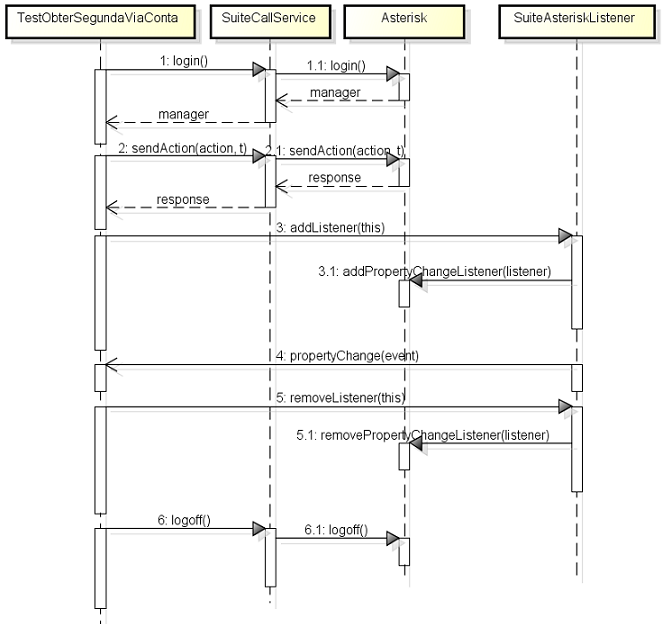
\includegraphics{figuras/diagramaSequencia.png}
	\legend {\fontsize{10}{12}\selectfont {Fonte: Autoria Própria}.}
\end{figure}

Durante a execução de um cenário de teste, é necessário monitorar o comportamento da chamada ou canal internamento na ferramente Asterisk,
afim de validar o retorno obtido pela requisição e posteriormente evidenciar a ocorrência do comportamento esperado ou de falhas. Com isso se faz necessário habilitar a conexão remota na ferramenta Asterisk. O arquivo \textit{/etc/asterisk/manager.conf} contém as propriedades necessárias para serem configuradas, abaixo é demostrado a configuração realizada para execução dos testes automatizados;
\\
\hspace{10 mm}\textit{[general]} 			\hspace{10 mm} $\triangleright$ Contexto geral de conexão.\\
\hspace{10 mm}\textit{enabled=yes}  		\hspace{10 mm} $\triangleright$ Habilitar a conexão remota.\\
\hspace{10 mm}\textit{port=5038}  			\hspace{10 mm} $\triangleright$ Define a porta.\\
\hspace{10 mm}\textit{displayconnects=yes}  \hspace{10 mm} $\triangleright$ Define a exibição das conexões no console.\\
\hspace{10 mm}\textit{permit=0.0.0.0/0.0.0.0} \hspace{10 mm} $\triangleright$ Define o endereço IP que será aceito.\\

Abaixo segue o exemplo de configuração para adição de um novo usuário para conexão remota;
\\
\hspace{10 mm}\textit{[manager]} 	\hspace{10 mm} $\triangleright$ Nome do novo usuário.\\
\hspace{10 mm}\textit{secret=pa55w0rd} \hspace{10 mm} $\triangleright$ Senha do novo usuário \\
\hspace{10 mm}\textit{read=system,call,log,verbose,command,agent}  \hspace{10 mm} $\triangleright$ Define as permissões de leitura.\\
\hspace{10 mm}\textit{write=system,call,log,verbose,command,agent}  \hspace{10 mm} $\triangleright$ Define as permissões de escrita.\\
\hspace{10 mm}\textit{permit=0.0.0.0/0.0.0.0} \hspace{10 mm} $\triangleright$ Define o endereço IP que será aceito \\


A distribuição Disc-OS por padrão possui uma configuração de firewall bastante restritiva por questões de segurança, para que não ocorra rejeição nas solicitações realizadas ao Asterisk, será para fins de testes desabilitada as regras do firewall, utilizando o seguinte comando \textit{/etc/init.d/iptables stop}.
 
 
% Figura para demonstrar a classe de teste - classe_teste_suite.png
% Para execução dos testes foi necessário realizar algumas customizações na ferramenta Asterisk, 
% desabilitar o iptables, 
% contexto de teste,
% Criação/Habilitar o user manager para remote conection.
% /etc/asterisk/manager.conf


